\chapter{Recurrent Neural Network}


\section{Definition}

The idea behind RNN is that in sequence prediction, the output $\selectonesample{x}{t+1}$ depends on all $\selectonesample{x}{i \leq t}$. So we need to calculate $p(\selectonesample{x}{t+1}|\selectonesample{x}{t}, \cdots, \selectonesample{x}{1})$. It is easier to simplify $p$ so the calculation could become $p(\selectonesample{x}{t+1}|\selectonesample{h}{t})$. Here $\selectonesample{h}{t} = f(\selectonesample{x}{t}, \cdots, \selectonesample{x}{1})$. $f$ could be simplified further so it takes fixed number of parameters: $\selectonesample{h}{t} = f(\selectonesample{x}{t}, \cdots, \selectonesample{x}{1}) = f(\selectonesample{x}{t}, \selectonesample{h}{t-1})$.

In both CNN and RNN, the model parameters are shared across different parts of the input. The difference is that
\begin{itemize}
    \item In CNN, the output depends on the neighbor of \emph{input}
    \item In RNN, the output depends on the neighbor of \emph{output}
\end{itemize}


\begin{example}[Fixed Size Output]
    In this example, the output size is the same as input size. Here $\selectonesample{h}{t}$ is the hidden state at time $t$ which is a fixed size vector. $\selectonesample{o}{t}$ is the output at time $t$ which is generated from hidden state.
    
\begin{equation}
    \begin{aligned}
        \selectonesample{h}{t} &= f\left(\selectonesample{h}{t-1}, \selectonesample{x}{t}; \theta\right) \\   
        \selectonesample{o}{t} &= g\left(\selectonesample{h}{t}\right)
    \end{aligned}    
\end{equation}

One concrete example is:

    \begin{equation}
        \begin{aligned}
            \selectonesample{h}{t} &= \tanh\left( W \selectonesample{h}{t-1} + U \selectonesample{x}{t} + b \right) \\
            \selectonesample{o}{t} &= \sigma \left(V \selectonesample{h}{t} + c\right)
        \end{aligned}
    \end{equation}    
\end{example}


We could put hidden layers on top of each other. The hidden state on layer $l$ at time $t$ depends on previous state and previous layer:
\begin{equation}
    \selectonesample{h_l}{t} = \varphi_l \left(W_{l-1} \selectonesample{h_{l-1}}{t} + W_l \selectonesample{h_l}{t-1} + b_l \right)
\end{equation}



There are 3 ways to construct RNN architecture:
\begin{enumerate}
    \item Recurrent connection is hidden state to the next hidden state
    \item Recurrent connection is from output to next hidden state
    \item Recurrent connection is from hidden state to another, and the output depends only on the last hidden state
\end{enumerate}

For these 3 architecture, the second one is weaker than the first one because the output is the training set target and it may not encode all the past history. 


It takes $O(t)$ to compute every backward step, so it requires $O(t^2)$ to finish backward propagation. Also because we need to keep all intermediate calculation result, the space cost is also $O(t)$. So it is wise to truncate the backward propagation sum to at most $k$ items.




% models
\section{Models}

\subsection{Vector to Vector Mapping}
When we generate from RNN, we sample from $\selectonesample{\tilde{y}}{t} \sim p(\selectonesample{y}{t}|\selectonesample{h}{t})$, and then determine the next hidden state $\selectonesample{h}{t+1} = f(\selectonesample{h}{t}, \selectonesample{\tilde{y}}{t}, x)$    


\subsection{Bidirectional RNN}

\begin{equation}
    \begin{aligned}
        h_t^{\rightarrow} &= \varphi(W_{xh}^{\rightarrow} x_t + W_{hh}^{\rightarrow} h_{t-1}^{\rightarrow} + b_h^{\rightarrow}) \\
        h_t^{\leftarrow} &= \varphi(W_{xh}^{\leftarrow} x_t + W_{hh}^{\leftarrow} h_{t-1}^{\leftarrow} + b_h^{\leftarrow})    \\
        y_t &= f(h_t^{\rightarrow}, h_t^{\leftarrow})
    \end{aligned}
\end{equation}

The training of bidirectional RNN needs skills:
\begin{itemize}
    \item In forward pass:
        \begin{itemize}
            \item Generate forward state and backward state
            \item Generate output
        \end{itemize}
    \item In backward pass:
        \begin{itemize}
            \item Calculate output gradient
            \item Calculate forward and backward node gradient
            \item Update weights
        \end{itemize}
\end{itemize}

Typical use cases of bidirectional RNN are:
\begin{enumerate}
    \item Fill the missing word
    \item Machine translation
\end{enumerate}

Bidirectional RNN cannot be used to do projection because it need data in $t+1$.

% lstm
\subsection{LSTM}

RNN is very hard to train because the gradient could easily explode or vanish. So RRN is hard to remember long term memory. LSTM and GRU were proposed to solve the problem. Long Short-term memory (LSTM) is a RNN that tries to forget the past. By default RNN will remember the past. It has two data:
\begin{enumerate}
    \item $\selectonesample{c}{t}$: cell state
    \item $\selectonesample{h}{t}$: hidden state
\end{enumerate}


\begin{definition}[Default LSTM]
The default LSTM implementation has two gates:
\begin{enumerate}
    \item Forget gate
    \item Input gate
\end{enumerate}

The formula is:
\begin{equation}
    \begin{aligned}
        \begin{pmatrix}
            \selectonesample{f}{t} \\
            \selectonesample{i}{t} \\
            \selectonesample{o}{t} \\
            \selectonesample{\tilde{c}}{t}
        \end{pmatrix} &= \begin{pmatrix}
            \sigma \\
            \sigma \\
            \sigma \\
            \tanh
        \end{pmatrix} \circ \left( \begin{pmatrix}
            W_f & U_f \\
            W_i & U_i \\
            W_o & U_o \\
            W_c & U_c
        \end{pmatrix} \times \begin{pmatrix}
            \selectonesample{x}{t} \\
            \selectonesample{h}{t-1}
        \end{pmatrix} + \begin{pmatrix}
            b_f \\
            b_i \\
            b_o \\
            b_c
        \end{pmatrix} \right) \\
        \selectonesample{c}{t} &= \selectonesample{f}{t} \odot \selectonesample{c}{t-1} + \selectonesample{i}{t} \odot \selectonesample{\tilde{c}}{t} \\
        \selectonesample{h}{t} &= \selectonesample{o}{t} \odot \tanh(\selectonesample{c}{t})
    \end{aligned}
\end{equation}

\begin{figure}[H]
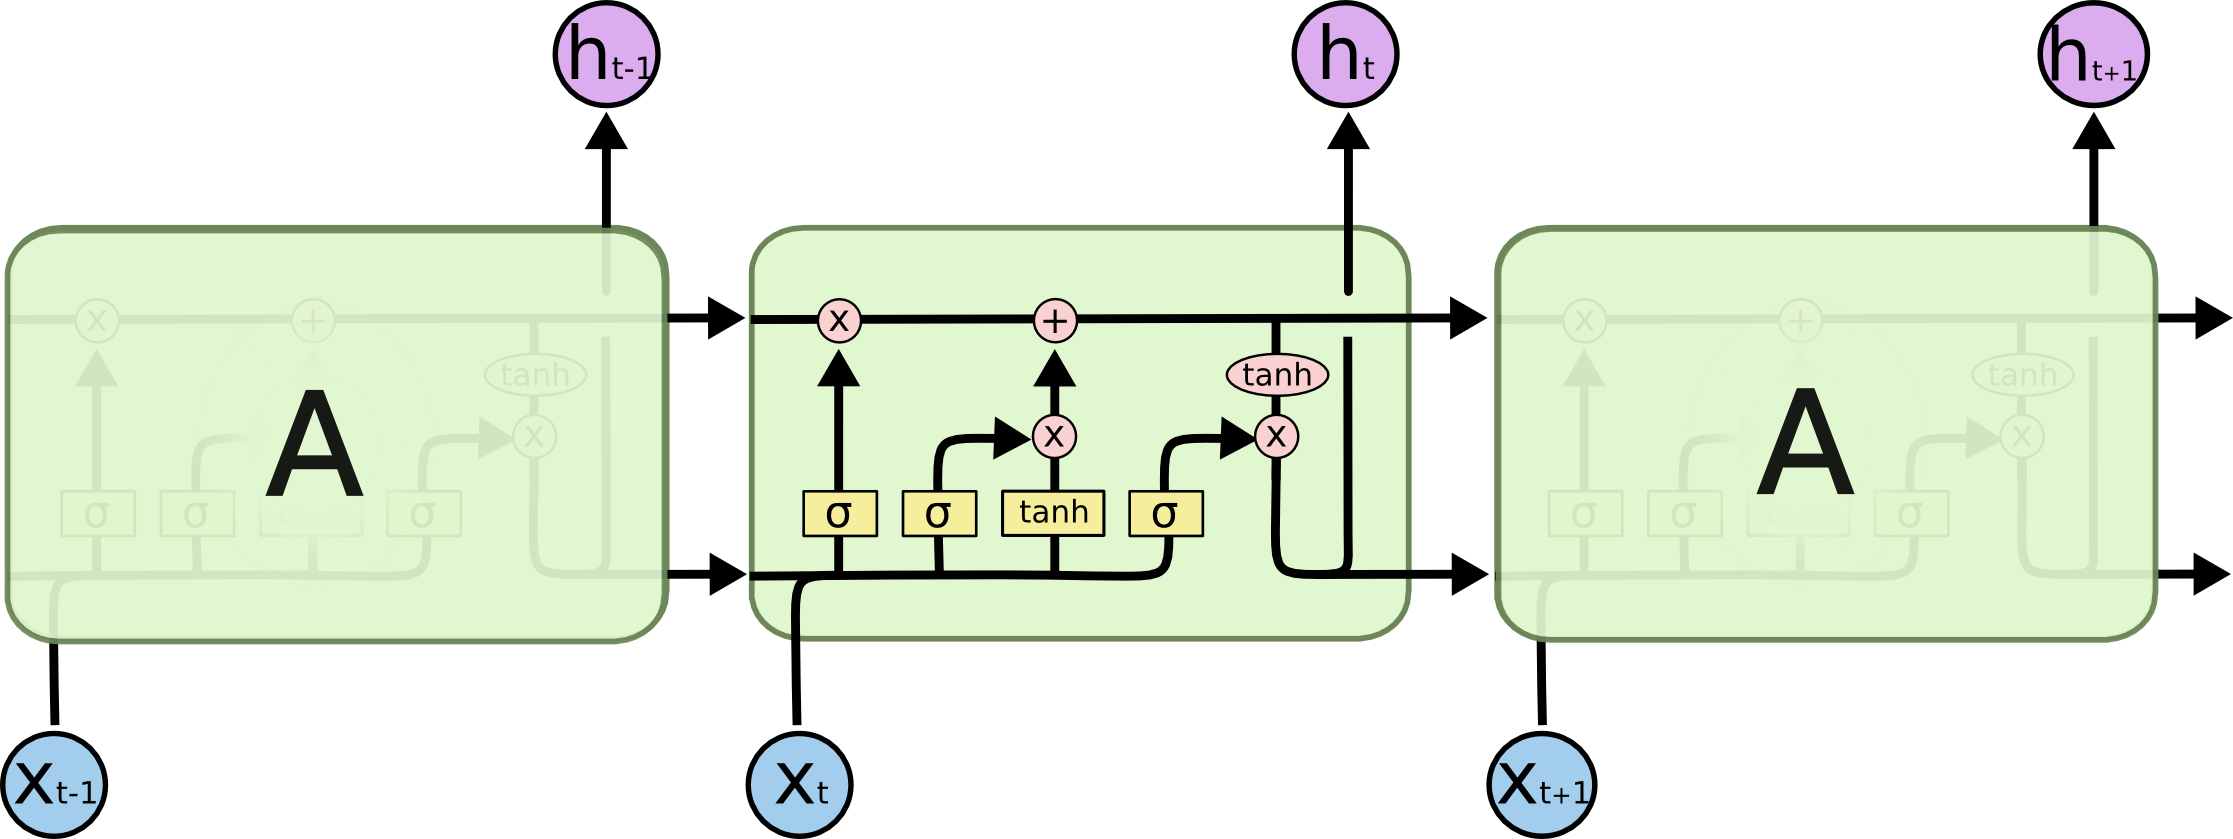
\includegraphics[width=0.8\textwidth]{machine_learning/pic/04/LSTM3-chain.png}
\centering
\caption{Default LSTM Implementation}
\end{figure}

\end{definition}


In default definition, $\selectonesample{f}{t}$ controls how much $\selectonesample{c}{t-1}$ to forget, and $\selectonesample{i}{t}$ controls how much to add. So the LSTM could keep long term memory if $\selectonesample{f}{t} = 1$ and $\selectonesample{i}{t} = 0$.

The initialization of forget gate needs to be careful. $b_f$ needs to be bigger enough, or the performance will be poor.

The shape of the variables are ($d$ is the input dimension and $h$ is the hidden unit dimension):
\begin{itemize}
    \item $\selectonesample{x}{t} \in \realnumber^d$: the input vector to LSTM
    \item $\selectonesample{f}{t} \in (0,1)^h$: forget gate's activation vector
    \item $\selectonesample{i}{t} \in (0,1)^h$: input gate's activation vector
    \item $\selectonesample{o}{t} \in (0,1)^h$: output gate's activation vector
    \item $\selectonesample{h}{t} \in (-1,1)^h$: hidden state vector
    \item $\selectonesample{\tilde{c}}{t} \in (-1,1)^h$: cell input activation vector
    \item $\selectonesample{c}{t} \in \realnumber^h$: cell state vector
\end{itemize}

LSTM is often initialized with $\selectonesample{c}{0} = \selectonesample{h}{0} = 0$.



\begin{definition}[Peephole LSTM]
    One famous variant is to let gate layers look at cell state:
    \begin{figure}[H]
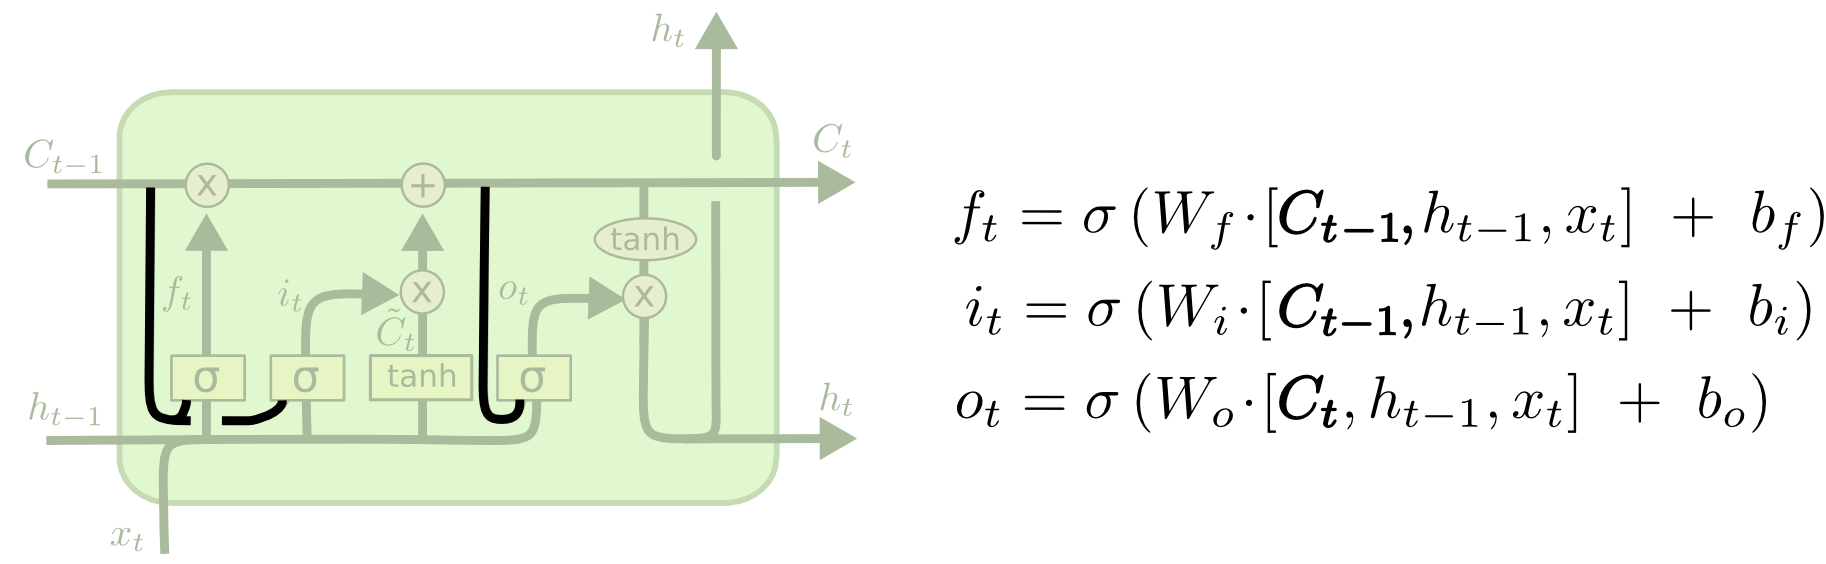
\includegraphics[width=0.8\textwidth]{machine_learning/pic/04/LSTM3-var-peepholes.png}
\centering
\caption{Peephole LSTM Implementation}
\end{figure}
\end{definition}

\begin{definition}
    In another variant, the forget gate and input gate are coupled. $\selectonesample{f}{t}$ controls how much to forget and $1- \selectonesample{f}{t}$ controls how much to input:
    \begin{figure}[H]
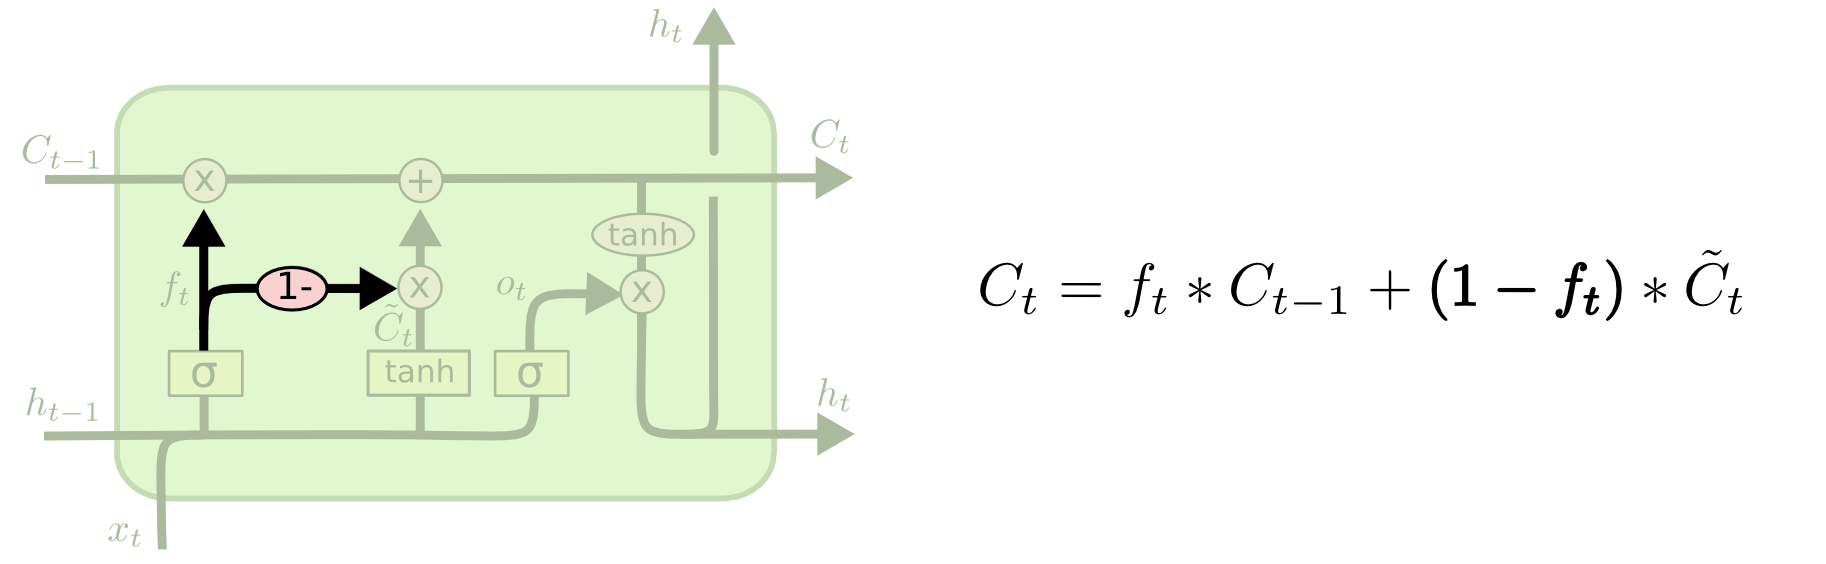
\includegraphics[width=0.8\textwidth]{machine_learning/pic/04/LSTM3-var-tied.png}
\centering
\caption{Coupled Forget and Input Gate}
\end{figure}
\end{definition}


\begin{definition}[GRU]
    GRU further simplified LSTM. It combines the forget and input gate into a single update gate. It also merges the cell state and hidden state.
\begin{figure}[H]
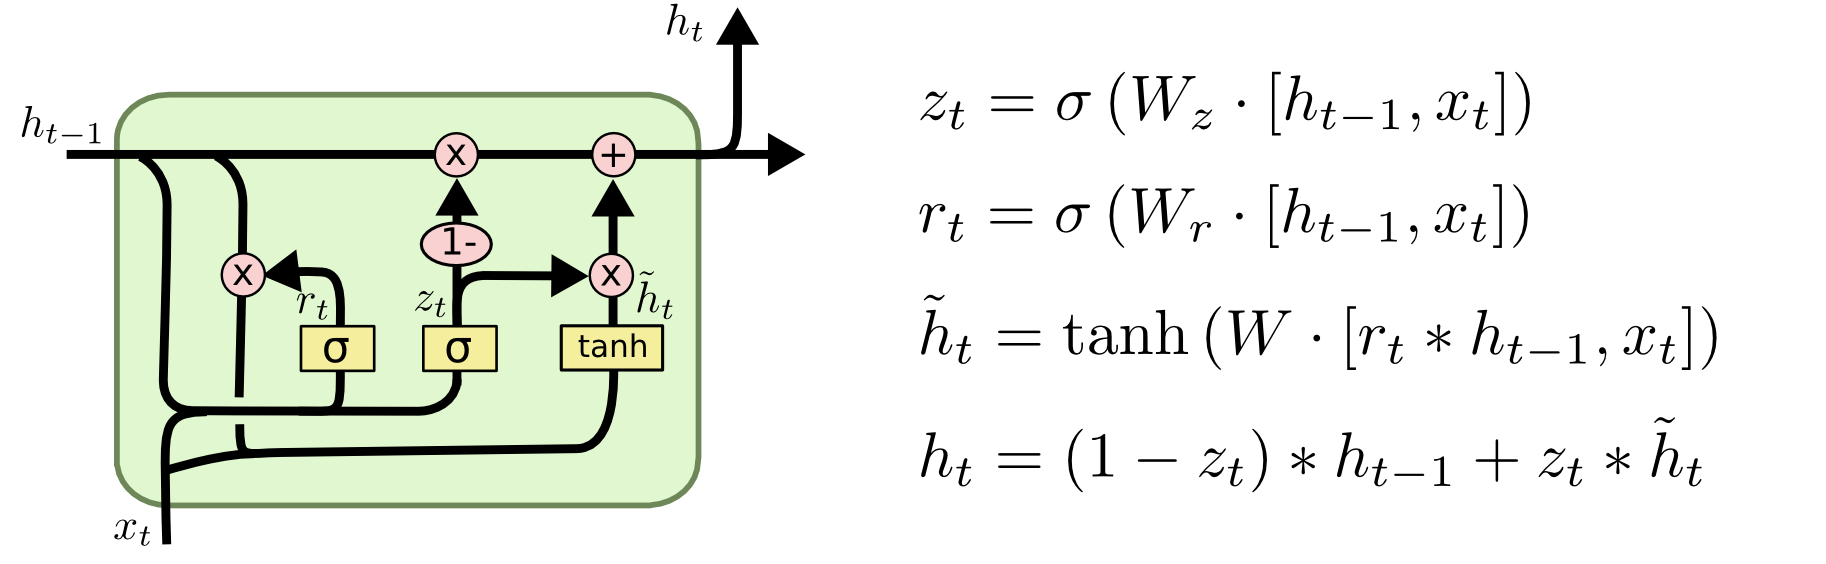
\includegraphics[width=0.8\textwidth]{machine_learning/pic/04/LSTM3-var-GRU.png}
\centering
\caption{GRU Implementation}
\end{figure}
\end{definition}



\subsection{Encoder Decoder}

it maps fixed-length input to a different length output.

the encoder is a stack of recurrent unit. the output is a vector of hidden state
\begin{equation}
    \selectonesample{h}{t} = \varphi \left(W \selectonesample{h}{t-1} + U \selectonesample{x}{t} \right)
\end{equation}

the output of the encoder hidden state is the initial hidden state of decoder. Because decoder does not have $x$, it will generate output purely based on hidden state:
\begin{equation}
    \selectonesample{h}{t} = f \left(W \selectonesample{h}{t-1} \right)
\end{equation}

We need to specify special word as the beginning and end of the sequence.

the problem with encoder-decoder are:
\begin{itemize}
    \item The hidden state size is fixed
    \item The next hidden state depends on previous hidden state
\end{itemize}
These problems make it difficult to learn long sentences and slow to learn.

Because the model takes output as input, it is also called \emph{auto-regressive}.

\subsection{Attention}

Attention optimize encoder-decoder by allowing decoder to access all encoder's hidden status. It effectively pass information from encoder to decoder.

\begin{figure}[H]
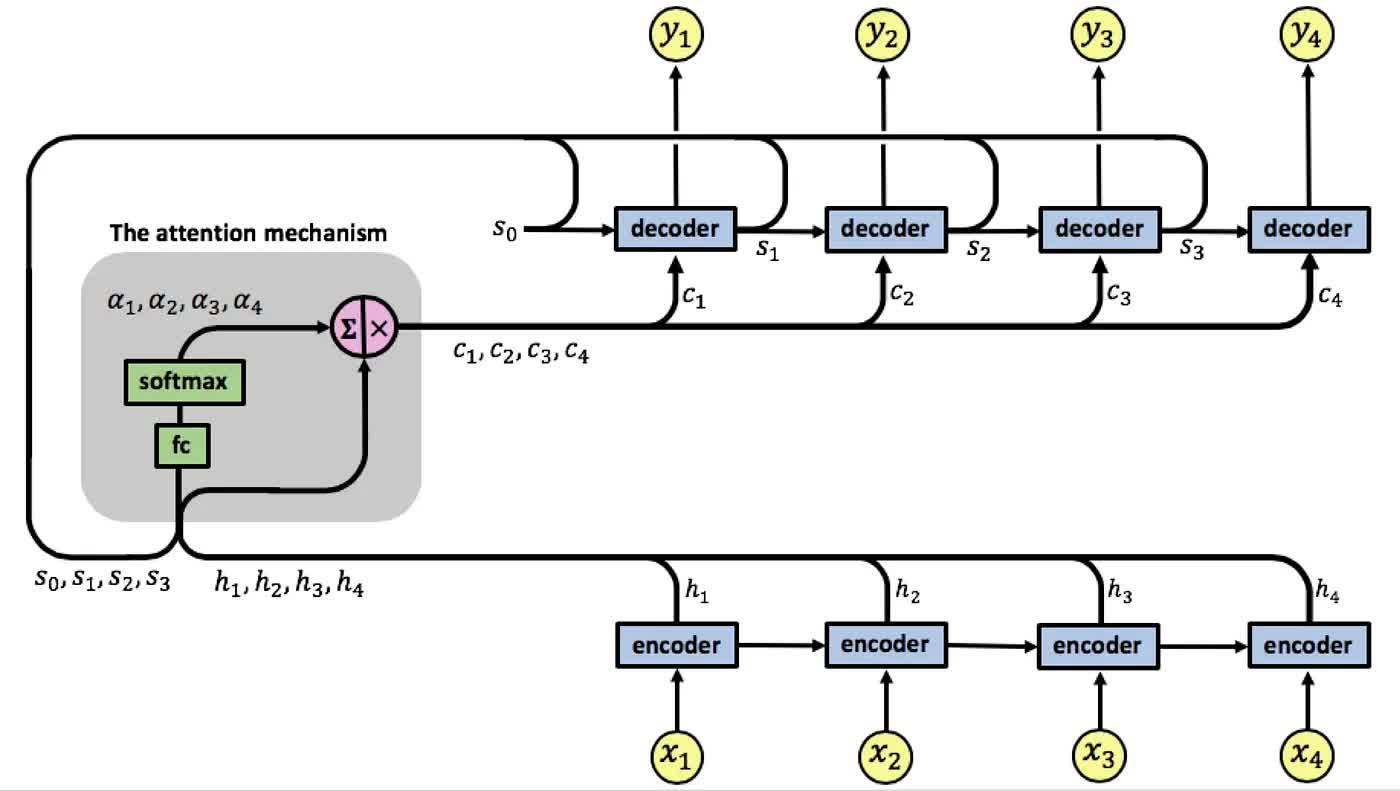
\includegraphics[width=0.8\textwidth]{machine_learning/pic/04/attention.jpeg}
\centering
\caption{Attention}
\end{figure}


As the picture above shows, the attention takes two inputs:
\begin{enumerate}
    \item All the outputs of encoder
    \item All the hidden status of decoder
\end{enumerate}

It will generate a sequence of vectors called context vectors. For each $s_i$ in the decoding layer ($i$ from $0$ to $4$, one by one):
\begin{enumerate}
    \item Calculate all $h_j$
    \item Combine $h_j$ and $s_i$ into a vector $[h_j, s_i]$ and pass to fully connected layer $\mathrm{fc}$ to get $e_{ij}$
    \item Apply softmax on $e_{ij}$ to produce $\alpha_i$
    \item Use weighted sum on $\alpha_i$ to create $c_i$
    \item Generate $s_{i+1}$ using $s_i$ and $c_i$. And iterate again
\end{enumerate}


 These $a_{ij}$ is learned using a fully connected network $\mathrm{fc}$ and softmax. Each context vector is a weighted sum of encoder's output:
\begin{equation}
    \begin{aligned}
        e_{ij} &= \mathrm{fc}(s_{i-1}, h_j) \\
        \alpha_{ij} &= \frac{\exp(e_{ij})}{\displaystyle \sum_{k=1}^4 \exp(e_{ik})} \\
        c_i &= \sum_{j=1}^4 \alpha_{ij} h_j
    \end{aligned}
\end{equation}


\subsection{Transformer}

\begin{definition}[Parametric Attention]
    Transformer makes a more generic argument on attention. The $s_i$ is the query, and $h_j$ is both the key and value. For each query $q$ and for all keys $k_j$.

\begin{equation}
    \begin{aligned}
        e_{ij} &= \frac{q \cdot k_j}{\sqrt{d_k}} \\
        \alpha_{ij} &= \frac{\exp(e_{ij})}{\displaystyle \sum_{k=1}^{T_x} \exp(e_{ik})} \\
        \mathrm{attention}(q, K, V) &= \sum_{j=1}^{V} a_{ij} v_j
    \end{aligned}
\end{equation}

There are new names for variables:
\begin{itemize}
    \item $d_k$ is the dimension of the query and key vector. $\sqrt{d_k}$ is used to stop softmax from generating small gradients
    \item $\alpha_{ij}$: attention weight
    \item $\mathrm{attention}(q, K, V)$: attention vector
\end{itemize}

For a batch of query $Q$, the calculation could be expressed in vector form:
\begin{equation}
    \mathrm{attention}(Q, K, V) = \mathrm{softmax}\left( \frac{Q \transpose{K}}{\sqrt{d_k}} \right)
\end{equation}
\end{definition}


\begin{definition}[Self-attention]
    In self-attention, the query is $x_i$, the keys and values are $(x_j, x_j)$. So the encoder attends to itself. At training time, because all the outputs are knows, the function could be evaluated in parallel, which is faster than sequential bottleneck of RNN.
\end{definition}

\begin{definition}[Multi-headed Attention]
    Multi-head Attention is a module for attention mechanisms which runs through an attention mechanism several times in parallel. The independent attention outputs are then concatenated and linearly transformed into the expected dimension.
    
    Intuitively, multiple attention heads allows for attending to parts of the sequence differently (e.g. longer-term dependencies versus shorter-term dependencies). This is the same as the multiple feature technique used in CNN.

\begin{figure}[H]
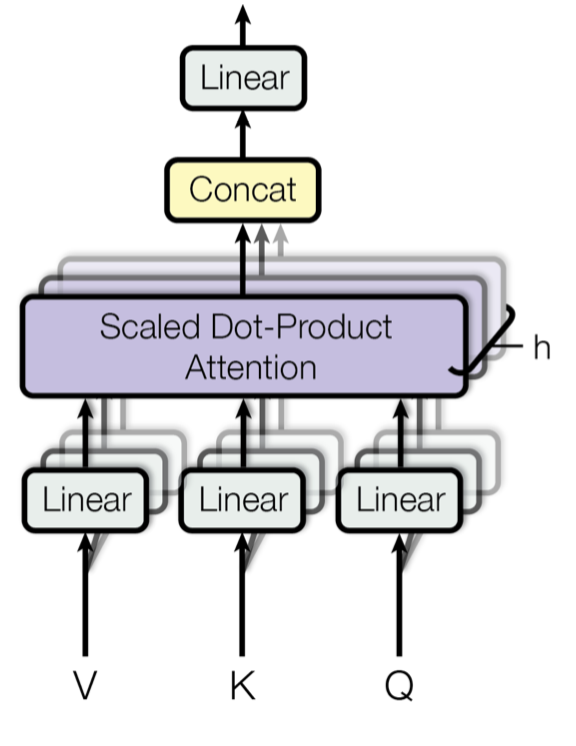
\includegraphics[width=0.3\textwidth]{machine_learning/pic/04/multi-headed-attention.png}
\centering
\caption{Multi-headed Attention}
\end{figure}
\end{definition}

\begin{equation}
    \begin{aligned}
        h_i &= \mathrm{attention}(Q W_q, K W_k, V W_v ) \\
        h &= W_0 \times \begin{pmatrix}
            h_1 & h_2 & \cdots & h_h
        \end{pmatrix}
    \end{aligned}
\end{equation}


\begin{definition}[Positional Encoding]
    Position encoding is an encoding of word position. Assume we want to encode the position $t$ using $d$ dimension, the new encoding is:
    \begin{equation}
        \begin{aligned}
            p_i (t) = \begin{cases}
            \displaystyle \sin\left(\frac{1}{C^{\frac{2k}{d}}} \cdot t \right)  \textrm{, if }  i = 2k \\
            \displaystyle \cos\left(\frac{1}{C^{\frac{2k}{d}}} \cdot t \right)  \textrm{, if }  i = 2k +1 \\
            \end{cases}
        \end{aligned}        
    \end{equation}
    
    Here $C$ is the maximum sequence length, which is usually $10,000$.
\end{definition}


Transformer used encoder-decoder architecture. In training time, the destination data will be shifted to the right and then feed into the output channel. In prediction time there is no input to the output channel.

The first layer is embedding layer, which change from a word into a vector.

The first layer of output channel is masked multi-headed attention. Because the output of attention could access all input and improper for output of time $t$ to see input after time $t$, there is a mask on input data to avoid seeing too much.

the self-attention layer will learn all the information in input. Because each output of the self-attention layer contains all information, we could apply MLP on top of each vector. In RNN, the information is passed from previous input to another, which self-attention aggregate all information at once.

another challenge is the order of time. in RNN, there is a natural order because next one depends on previous one. For self-attention, all information were processed at once and there is no order information. 





























































































































































































































































































































































































































